\section{Overlay Accelerator Framework}
A block diagram of the proposed overlay accelerator system, based on an array of linear TM overlays~\cite{li2018time}, which supports both Zynq-based SoC and standalone PCIe accelerators, is shown in Figure~\ref{system}. 
The FPGA memory subsystem provides the interface between the overlay on the FPGA fabric and the ARM processor on a Zynq SoC via the AXI bus (or directly to the memory via the PCIe link). 
For the AXI bus-based overlay, two 32-bit FIFOs are used to connect a single 32-bit linear TM overlay with the memory subsystem. 
%For the PCIe-based overlay, four 32-bit linear TM overlays are used to make full use of the 128-bit data bandwidth and thus reduce the II to a quarter of that of a single overlay. 
For the PCIe-based overlay, we propose replicating four 32-bit linear TM overlays to make full use of the 128-bit data bandwidth. The four overlay instances can implement multiple compute kernels at runtime and thus reduce the II to a quarter of that of a single overlay.
Data transfers between the internal memory subsystem, the DDR SDRAM and the offchip DRAM are under the control of a scatter-gather DMA engine. 
%The overlays are connected to the memory subsystem via two 128-bit FIFOs. 

\begin{figure}[tb]
	\centering
	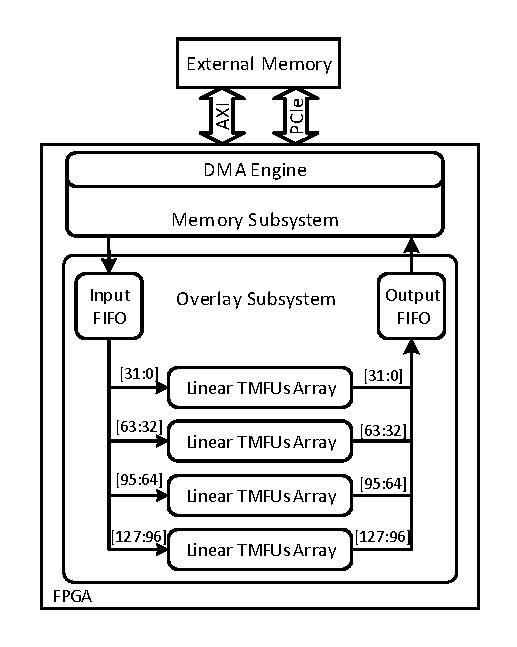
\includegraphics[width=\columnwidth]{Figures/system_new.pdf}
	\caption{The proposed overlay accelerator system.}
	\label{system}
\end{figure}

%\begin{figure}
%	\centering
%	\subfigure[Block diagram of the system]{
%	\centering
%	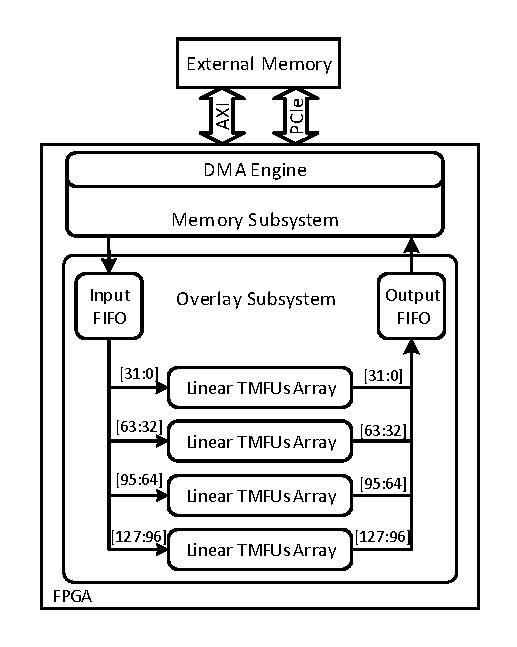
\includegraphics[width=0.9\columnwidth]{Figures/system_new.pdf}
%	\label{a}
%	}
%	~
%	\subfigure[A linear TM overlay]{
%	\centering
%	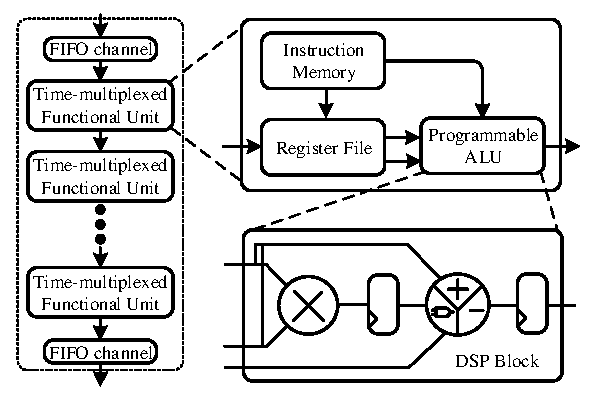
\includegraphics[width=0.9\columnwidth]{Figures/overlay.pdf}
%	\label{b}
%	}
%	\caption{The proposed overlay accelerator system.}
%	\label{system} %% label for entire figure
%\end{figure}


\subsection{Xillybus}
Xillybus is a portable, easy to use DMA-based data transfer solution which provides a simple abstraction of the AXI/PCIe interfaces. 
%There is no prerequisite for knowledge of the AXI or PCIe protocols as all the low-level design is packaged into an IP core. 
One side of the Xillybus IP core is connected to the host processor, while the other side communicates with two standard FIFOs, providing six signals to control the data flow, as shown in Figure~\ref{xillybus}. 
The host processor can be either the ARM processor of the Xilinx Zynq SoC (AXI-Xillybus: for an AXI bus-based solution) or a PC based x86 CPU (PCIe-Xillybus: for a PCIe-based solution). 

\begin{figure}[tb]
	\centering
	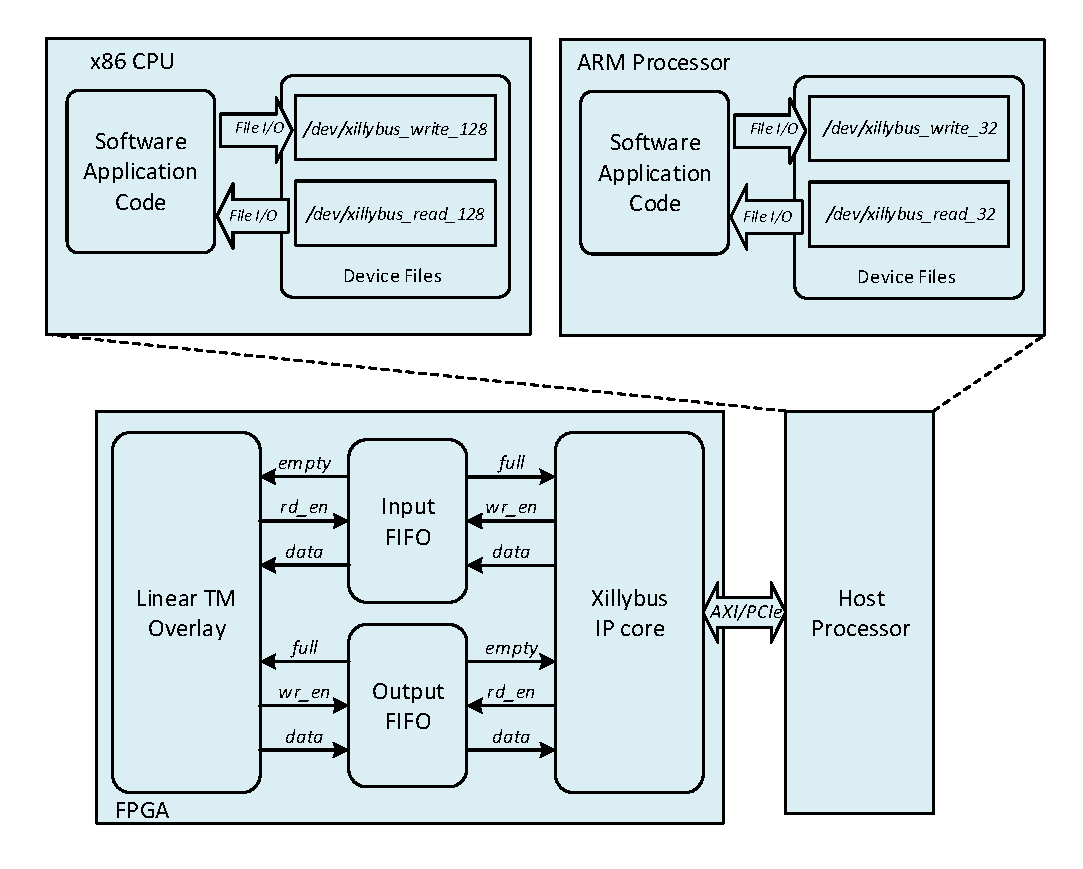
\includegraphics[width=0.9\columnwidth]{Figures/xillybus.pdf}
	\caption{Xillybus-based overlay accelerator.}
	\label{xillybus} 
\end{figure}


\begin{comment}
Xillybus provides a simple data loopback demo design (\textit{xillydemo.v}).   
After the driver installation and the FPGA is programmed by the Xillybus bitstream, several device files such as \textit{/dev/xillybus\_write\_32(128)} and \textit{/dev/xillybus\_read\_32(128)} are generated by the host driver which can be read from and written to like any file using basic Linux commands such as \textit{write} and \textit{read}. 
Xillybus also provides an IP core factory for users to customize multiple streaming device files and seekable device files which have access to the standard FPGA RAM. 
\end{comment}


\subsection{RIFFA}
RIFFA has a more complicated framework which consists of three layers, as shown in Figure~\ref{riffa}. 
%It can be visually divided into two part, one part containing the device driver and the software APIs in the PC while the other one including all the PCIe hardware interface design in the FPGA. 
%A vendor-specific PCIe endpoint bridges the connection between RIFFA and host CPU via the PCIe link. 
%It is mainly comprised of three layers. 
On the bottom layer, an RX engine and a TX engine are connected to the vendor-specific PCIe Endpoint IP core, which bridges the connection between RIFFA and the host CPU. 
The middle layer supports up to 12 channels which send packets to the TX engine and receive packets from the RX engine through a scatter-gather DMA engine. 
The overlay which connects to the RX/TX FIFOs from the communication channels, is located on the top layer. 

\begin{figure}[tb]
	\centering
	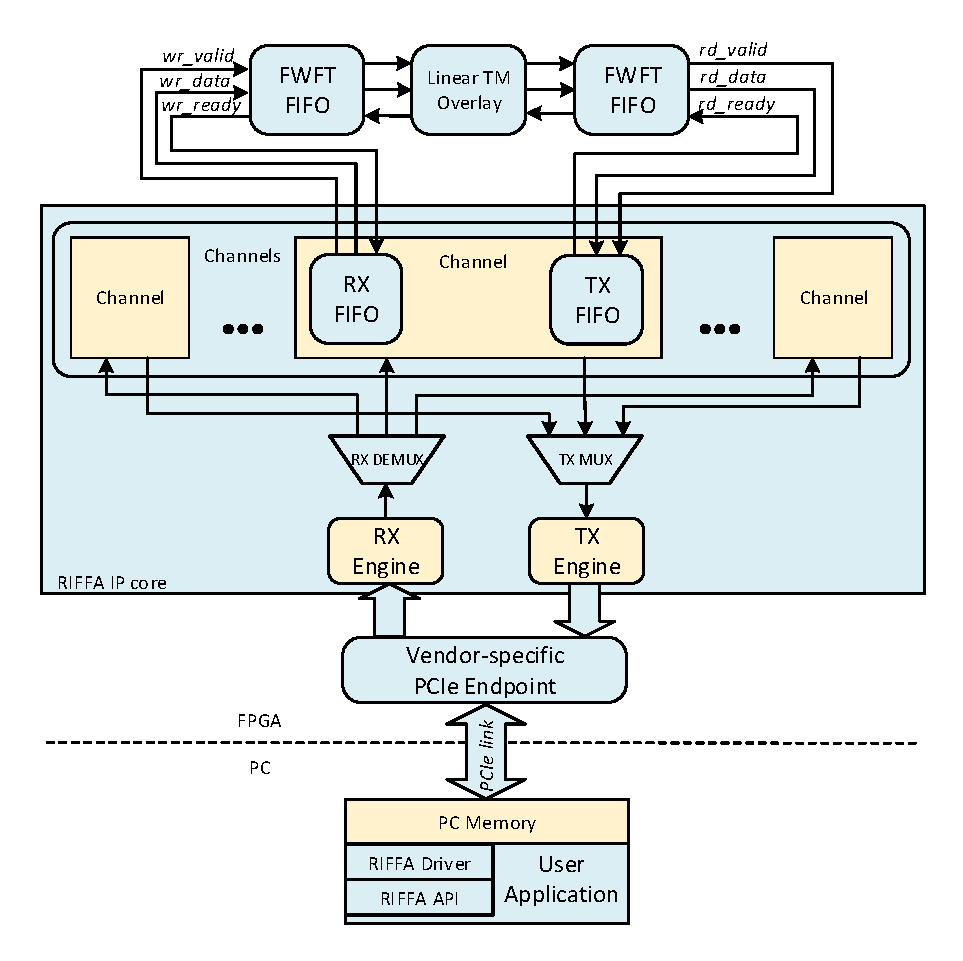
\includegraphics[width=0.9\columnwidth]{Figures/riffa.pdf}
	\caption{RIFFA-based overlay accelerator.}
	\label{riffa}
\end{figure}


\begin{comment}
An example design for data transfer (\textit{chnl\_test.v}), along with driver and software code (\textit{testutil.c}), is provided.
A single channel is used to receive data from the host via the RX engine and send the same amount of data back to the host via the TX engine. 
Dedicated software APIs (\textit{fpga\_send} and \textit{fpga\_recv}) were developed as blocking functions.
%For a more complicated design, multiple channels (up to 12 per FPGA) can be instantiated to integrate with different user cores independently. 
\end{comment}


\subsection{DyRACT}
The original version of DyRACT communication infrastructure enables PCIe-based high-speed communication between a host computer and FPGA-based user logic with support for partial reconfiguration (PR). 
It provisions multiple AXI4-stream backend interface, enabling seamless integration with vendor-supported IP cores. 
We have modified the original version to make it lite-weight and tailored to support the proposed overlay architecture. 
Since the present implementation does not exploit PR, the reconfiguration control logic is disabled, and a single backend AXI4-stream interface is enabled. 
The stream interface width is configurable through width-conversion FIFOs. 
A new AXI-Lite interface is added to support command-data interface between the host and the overlay.
The software architecture follows similar structure of that of RIFFA. 
The low-level communication protocols and interrupts are managed by the driver and the user library provides APIs for integration with application programmes. 

\subsection{Programming Model}
